\documentclass[a4paper,11pt,cours]{nsi} % COMPILE WITH DRAFT
\geometry{margin=2cm}
\usepackage{hyperref}
\usepackage{yhmath}

\begin{document}

\setcounter{chapter}{7} % 1 de moins que le num de chapitre



\chapter{Fonctions dérivées et applications}


\setlength{\columnseprule}{0.5pt}
\setlength{\columnsep}{1cm}

\section{Fonction dérivée}
\begin{definition}
	Soit $f$ une fonction définie sur un intervalle \textbf{ouvert} $I$.\\
	Si $f$ est dérivable en tout nombre de $I$ alors on dit que $f$ est 
	{\boldmath\textbf{dérivable \emph{sur} $I$}}. On peut alors définir la {\boldmath\textbf{fonction dérivée de $f$}} (aussi appelée la dérivée 
	de $f$, plus simplement) : à tout nombre $x$ de $I$ elle associe $f'(x)$, le nombre dérivé de $f$ en $x$.
\end{definition}

\begin{exemple}[ 1]
	La fonction $f$ définie sur $\R$ par $f(x)=3x-2$ est dérivable sur $\R$. En effet , soit $x\in\R$ et soit $h\neq 0$, on a alors :
	\begin{tabbing}
		$\dfrac{f(x+h)-f(x)}{h}$	\=	$=\dfrac{3(x+h)-2-(3x-2)}{h}$\\
		\>	$=\dfrac{3h}{h}$\\	
		\>	$=3$
	\end{tabbing}
	Ainsi quand $h$ tend vers zéro cette quantité tend vers $3$ (bien évidemment vu qu'elle ne dépend pas de $h$). On a donc $f'(x)=3$.\\
	$f'$ est donc la fonction constante qui à tout réel $x$ associe $3$.\\
	Ce n'est pas très étonnant vu que la représentation graphique de $f$ est une droite de pente $3$ (elle est sa propre tangente en tout point).
\end{exemple}

\begin{exemple}[ 2]
	La fonction $g$ définie sur $\R$ par $g(x)=3x^2-4x+1$ est dérivable sur $\R$ : \\
	Soit $x\in\R$ et soit $h\neq 0$, on a alors :
	\begin{tabbing}
		$\dfrac{g(x+h)-g(x)}{h}$	\=	$=\dfrac{3(x+h)^2-4(x+h)+1-(3x^2-4x+1)}{h}$\\
		\>	$=\dfrac{3x^2+6xh+3h^2-4x-4h+1-3x^2+4x-1}{h}$\\	
		\>	$=\dfrac{6xh-4h+3h^2}{h}$\\
		\>	$=6x-4+3h$
	\end{tabbing}
	Quand $h$ tend vers zéro cette quantité tend vers $6x-4$. On a donc $f'(x)=6x-4$.\\
	$f'$ est donc la fonction affine définie par $f'(x)=6x-4$.
\end{exemple}


\subsection*{Dérivées des fonctions de référence}
\begin{propriete}[ ]
	On note $D_f$ l'ensemble de définition de la fonction $f$ et $D_{f'}$ son ensemble de dérivabilité.\\
	
	\renewcommand{\arraystretch}{2}
	\begin{tabular}{|c|c|c|c|}
		\hline
		\textbf{Fonction $f$ définie par :} & $D_f$ & \textbf{Fonction dérivée $f'$ définie par :} & $D_{f'}$\\
		\hline
		
		$f(x)=k$, avec $k\in \R$ & $\R$ & $f'(x)=0$ & $\R$ \\
		\hline
		$f(x)=mx+p$, avec $m,p \in \R$ & $\R$ & $f'(x)=m$ & $\R$ \\
		\hline
		$f(x)=x^2$ & $\R$ & $f'(x)=2x$ & $\R$ \\
		\hline
		$f(x)=x^n$, avec $n\in \N^*$ & $\R$ & $f'(x)=nx^{n-1}$ & $\R$ \\
		\hline
		$f(x)=\dfrac{1}{x}$ & $\R \backslash \{0\}$ & $f'(x)=-\dfrac{1}{x^2}$ & $\R\backslash \{0\}$ \\
		\hline
		$f(x)=\dfrac{1}{x^n}$, avec $n\in \N^* $& $\R \backslash \{0\}$ & $f'(x)=-\dfrac{n}{x^{n+1}}$ & $\R\backslash \{0\}$ \\
		\hline
		$f(x)=\sqrt{x}$ & $\fio{0}{+\infty}$ & $f'(x)=\dfrac{1}{2\sqrt{x}}$ & $\oio{0}{+\infty}$\\
		\hline
	\end{tabular}
\end{propriete}

Il est important de connaître ce tableau \textbf{par cœur} pour ne pas avoir à recalculer des limites de taux de variation comme dans les exemples 1 et 2. Cela nous fera gagner beaucoup de temps par la suite.

\section{Fonctions dérivées et opérations}
Pour ce paragraphe, $u$ et $v$ désignent deux fonctions définies et dérivables sur un même intervalle ouvert $I$.
\subsection{Dérivée d'une somme}

\begin{propriete}[]
	La fonction $u+v$ est dérivable sur $I$ et l'on a :$${\boldmath\boxed{(u+v)'=u'+v'}}$$
\end{propriete}
\begin{demonstration}
	\carreauxseyes{16}{1.6}\\	
    \newpage
    \carreauxseyes{16}{6.4}
\end{demonstration}

\begin{exemple}[]
	La fonction $f$ définie sur $\R^*_+$ par $f(x)=x^2+3x+\sqrt{x}$ est dérivable sur $R^*_+$, de dérivée\\ $f'(x)=2x+3+\dfrac{1}{2\sqrt{x}}$.
\end{exemple}

\subsection{Dérivée d'un produit}

\begin{propriete}[] 
	La fonction $uv$ est dérivable sur $I$ et l'on a :$${\boldmath\boxed{(uv)'=u'v+uv'}}$$
\end{propriete}
\begin{demonstration}
	\carreauxseyes{16}{9.6}
\end{demonstration}

\begin{exemple}
	La fonction définie sur $\R^*_+$ par $f(x)=x^2\sqrt{x}$ est dérivable sur cet intervalle de dérivée :
	\begin{tabbing}
		$f'(x)$	\=	$=2x\times \sqrt{x}+x^2\times \dfrac{1}{2\sqrt{x}}$\\
		\>	$=2x\sqrt{x}+\dfrac{x^2}{2\sqrt{x}}$\\
		\>	$=\dfrac{2x^2}{\sqrt{x}}+\dfrac{x^2}{2\sqrt{x}}$\\
		\>	$=\dfrac{4x^2}{2\sqrt{x}}+\dfrac{x^2}{2\sqrt{x}}$\\
		\>	$=\dfrac{5x^2}{2\sqrt{x}}$\\
		\>	$=\dfrac{5}{2}x\sqrt{x}$
	\end{tabbing}
\end{exemple}
\subsection{Dérivée d'un produit de fonction par un réel}
\begin{propriete}[]
	Soit $k$ un réel, alors la fonction $ku$ est dérivable sur $I$ et on a :$${\boldmath\boxed{(ku)'=ku'}}$$
\end{propriete}
\begin{demonstration}
	\carreauxseyes{16}{8}
\end{demonstration}	

\begin{exemple}[]
	La fonction définie sur $\R$ par $f(x)=7x^2$ a est dérivable sur $\R$ et a pour dérivée $f'(x)=14x$.	
\end{exemple}

\subsection{Dérivée du carré d'une fonction}
\begin{propriete}
	$u^2$ est dérivable sur $I$ et :$${\boldmath\boxed{(u^2)'=2uu'}}$$
\end{propriete}
\begin{demonstration}
	\carreauxseyes{16}{8}
\end{demonstration}
\begin{exemple}[]
	La fonction définie sur $\R$ par $f(x)=x^4$ (c'est à dire $f(x)=\left(x^2\right)^2$ est dérivable sur $R$ et
	\begin{tabbing}
		$f'(x)$	\=	$=2\times x^2\times 2x$\\
		\>	$=4x^3$
	\end{tabbing}	
\end{exemple}

\subsection{Dérivée de l'inverse d'une fonction}

\begin{propriete}[]
	Supposons que $u$ ne s'annule pas sur $I$ (c'est à dire que pour tout $x\in I$, $u(x)\neq 0$), alors la fonction $\dfrac{1}{u}$  est définie sur $I$. Elle est dérivable sur $I$ et :
	$${\boldmath\boxed{\left(\dfrac{1}{u}\right)'=-\dfrac{u'}{u^2}}}$$
\end{propriete}
\begin{demonstration}
	\carreauxseyes{16}{8.8}
\end{demonstration}
\begin{exemple}[]
	La fonction définie sur $]\ 2\ ;\ +\infty\ [$ par $f(x)=\dfrac{1}{2x-3}$ est dérivable sur cet intervalle et on a :
	$$f'(x)=-\dfrac{2}{(2x-3)^2}$$	
\end{exemple}

\subsection{Dérivée du quotient de deux fonctions}
\begin{propriete}
	Supposons que $v$ ne s'annule pas sur $I$, alors la fonction $\dfrac{u}{v}$ est définie sur $I$. Elle est dérivable sur $I$ et 
	:$${\boldmath\boxed{\left(\dfrac{u}{v}\right)'=\dfrac{u'v-uv'}{v^2}}}$$
\end{propriete}
\begin{demonstration}
	\carreauxseyes{16}{4}\\

    \carreauxseyes{16}{4.8}
\end{demonstration}

\begin{exemple}[]
	La fonction définie sur $\R$ par $f(x)=\dfrac{x^2}{x^2+1}$ est dérivable sur $\R$ et 
	\begin{tabbing}
		$f'(x)$	\=	$=\dfrac{2x\times(x^2+1)-x^2\times 2x}{(x^2+1)^2}$\\
		\>	$=\dfrac{2x^3+2x-2x^3}{(x^2+1)^2}$\\
		\>	$=\dfrac{2x}{(x^2+1)^2}$
	\end{tabbing}
\end{exemple}

\subsection{Dérivée de $f$ définie par $f(x)=g(ax+b)$}
\begin{propriete}[ ]
	Soient $a$ et $b$ deux réels et soit $J$ l'intervalle tel que pour tout $x\in J, ax+b \in I$.\\
	La fonction $f:x\mapsto g(ax+b)$ est définie et dérivable sur $J$ et :
		$${\boldmath\boxed{f'(x)=a\times g'(ax+b)}}$$
\end{propriete}

\begin{exemple}[ ]
	La fonction définie sur $\fio{-\dfrac{4}{3}}{+\infty}$ par $f(x)=\sqrt{3x+4}$ est dérivable sur $\oio{-\dfrac{4}{3}}{+\infty}$ et 
	\begin{tabbing}
		$f'(x)$ \=	$=3\times \dfrac{1}{2\sqrt{3x+4}}$\\[0.5em]
		\>	$=\dfrac{3}{2\sqrt{3x+4}}$
	\end{tabbing}
\end{exemple}

\section{Variations d'une fonction et dérivée}


\begin{propriete}[]
	Soit $f$ une fonction dérivable sur un intervalle $I$.
	\begin{enumerate}[label=\textbullet]	
		\item 	Si $f'=0$ sur $I$ alors $f$ est constante sur $I$.
		\item 	Si $f'\geqslant 0$ sur $I$ alors $f$ est croissante sur $I$.
		\item 	Si $f'\leqslant 0$ sur $I$ alors $f$ est décroissante sur $I$.
		\item 	Si $f'>0$ sur $I$ alors $f$ est strictement croissante sur $I$.
		\item 	Si $f'<0$ sur $I$ alors $f$ est strictement décroissante sur $I$.
	\end{enumerate}
\end{propriete}
\emph{Cette propriété est admise.}


\begin{remarque}[]
	Dans la propriété précédente, les réciproques des deux dernières affirmations sont fausses.\\
	En effet, par exemple, la fonction $x\mapsto x^3$ est strictement croissante sur $\R$ mais sa dérivée $x\mapsto 3x^2$ n'est pas strictement 
	positive sur $\R$ car elle s'annule en zéro.
\end{remarque}


\begin{definition}[s]
	Soit $f$ une fonction définie sur un intervalle $I$ et $c\in I$.
	\begin{enumerate}[label=\textbullet]
		\item 	On dit que $f$ admet un maximum sur $I$, atteint en $c$ si pour tout $x\in I$, $f(x)\leqslant f(c)$.\\
		Ce maximum vaut alors $f(c)$.
		\item 	On dit que $f$ admet un minimum sur $I$, atteint en $c$ si pour tout $x\in I$, $f(x)\geqslant f(c)$.\\
		Ce minimum vaut alors $f(c)$.
		\item 	Dans les deux cas on dit que $f$ admet un extrémum en $c$.
	\end{enumerate}
\end{definition}


\begin{definition}[]
	Soit $f$ une fonction définie sur un intervalle $I$.\\
	S'il existe un intervalle \textbf{ouvert }$J$ inclus dans $I$ et $c\in J$ tel que $f$ admette un extrémum sur $J$, on dit que $f$ 
	admet un extrémum local en $c$.
\end{definition}

\begin{remarque}[]
	Dans le cas ou $f$ admet un extrémum sur $I$ en $c$, on parle d'extremum global.\\
	Un extrémum global est un extrémum local.\\
	Un extrémum local n'est pas en général un extrémum global.
\end{remarque}

\begin{propriete}[]
	Soit $f$ une fonction dérivable sur un intervalle $I$ et $a\in I$.\\
	Si $f'$ s'annule en changeant de signe en $a$ alors $f$ admet un extrémum local en $a$.
\end{propriete}

\newpage

\begin{methode}[ : \'Etudier une fonction]
	\ \\
	On considère la fonction $f$ définie sur $\R$ par $f(x)=x^3-6x^2-15x+2$.\\
	
	\textbf{\boldmath 1. On explique pourquoi $f$ est dérivable et sur quel ensemble :}\\[.5em]	
	$f$ est dérivable sur $\R$ comme somme de fonction dérivables sur $\R$.\\
	
	\textbf{\boldmath 2. On détermine l'expression algébrique de $f'(x)$ :}\\[.5em]
	Pour tout$ x\in\R$, $f'(x)=3x^2-12x-15$\\
	
	\textbf{\boldmath 3. On étudie le signe de $f'$ :}\\[.5em]	
	$f'$ est un polynôme de degré 2, on détermine son discriminant, celui-ci vaut 324, donc $f'$ admet deux racines que l'on détermine par le calcul : -1 
	et 5. \'Etant donné que le coefficient de plus haut degré de $f'$ est positif, on obtient le tableau suivant :
	\begin{center}
		\begin{tikzpicture}
			\tkzTabInit[color,lgt=2,espcl=2]
			{$x$ /.7 ,$f'(x)$ /.7}
			{$-\infty$, -1 ,5, $+\infty$ }
			\tkzTabLine{,+ , z, -,z,+,}
		\end{tikzpicture}
	\end{center}
	\textbf{\boldmath 4. On en déduit les variations de $f$ :}
	\begin{center}
		\begin{tikzpicture}
			\tkzTabInit[color,lgt=2,espcl=2]
			{$x$ /.7 ,$f'(x)$ /.7,$f$ /1.4}
			{$-\infty$, -1 ,5, $+\infty$ }
			\tkzTabLine{,+ , z, -,z,+,}
			\tkzTabVar{-/,+/,-/,+/}
		\end{tikzpicture}
	\end{center}
	{\boldmath\textbf{5. On calcule la valeur de chaque extrémum de $f$ :}}\\[.5em]	
	On calcule que $f(-1)=10$ et que $f(5)=-98$. On reporte dans le \textbf{tableau final :}
	\begin{center}
		\begin{tikzpicture}
			\tkzTabInit[color,lgt=2,espcl=2]
			{$x$ /.7 ,$f'(x)$ /.7,$f$ /1.4}
			{$-\infty$, -1 ,5, $+\infty$ }
			\tkzTabLine{,+ , z, -,z,+,}
			\tkzTabVar{-/,+/10,-/-98,+/}
		\end{tikzpicture}
	\end{center}
	
	\begin{center}
		\def\xmin{-4} \def\ymin{-100}\def\xmax{8}\def\ymax{30}
		\def\F{(\x)^3-6*(\x)^2-15*\x+2}
		\begin{tikzpicture}[yscale=1/20]
			\clip (\xmin,\ymin) rectangle (\xmax,\ymax);
			\draw[fill=white](\xmin,\ymin) rectangle (\xmax,\ymax);
			
			\draw[xstep=1,ystep=10,quadrillage@color](\xmin,\ymin) grid (\xmax,\ymax);
			\draw[thick,->] (\xmin,0)--(\xmax,0);
			\draw[thick,->] (0,\ymin)--(0,\ymax);
			\draw[UGLiBlue,thick,domain=\xmin:\xmax,smooth,variable=\x] plot ({\x},{\F});
			\foreach \i in {-3,...,-1}{\draw(\i,0) node[below]{\i};}
			\foreach \i in {1,...,7}{\draw(\i,0) node[below]{\i};}
			\foreach \j in {-100,-80,...,-20}{\draw(0,\j) node[left]{\j};}
			\draw (0,20) node[left]{20};
		\end{tikzpicture}
	\end{center}
\end{methode}

\begin{exemple}[]
	\ \\
	{\boldmath\textbf{\'Etudier la fonction $g$ définie par $g(x)=x-\sqrt{x}$.}}\\
	
	\begin{enumerate}[label=\textbullet]
		\item 	$\mathcal{D}_g=\R_+$ car $x$ doit être positif pour pouvoir écrire $\sqrt{x}$.
		\item 	La fonction $g$ est dérivable sur $\R^*_+$ comme somme de fonction dérivable et sa dérivée est
		\begin{tabbing}
			$g'(x)$	\=	$=1-\dfrac{1}{2\sqrt{x}}$\\
			\\
			\>	$=\dfrac{2\sqrt{x}-1}{\sqrt{x}}$
		\end{tabbing}
		\item 	Pour étudier le signe de $g'(x)$, on remarque que son dénominateur est positif. On doit donc étudier le signe de son numérateur en 
		résolvant l'inéquation
		\begin{tabbing}
			$2\sqrt{x}-1>0\quad$	\=	$\Leftrightarrow\quad \sqrt{x}>\dfrac{1}{2}$\\
			\\
			\>	$\Leftrightarrow\quad \left(\sqrt{x}\right)^2>\left(\dfrac{1}{2}\right)^2$\\
			\\
			\>	$\Leftrightarrow\quad x>\dfrac{1}{4}$
		\end{tabbing}
		\item Sachant que $g\left(\dfrac{1}{4}\right)=\dfrac{1}{4}-\dfrac{1}{2}=-\dfrac{1}{4}$ on obtient le tableau suivant :\\
		\begin{center}
			\begin{tikzpicture}
				\tkzTabInit[color,lgt=2,espcl=2]
				{$x$ /.7 ,$g'(x)$ /.7,$g$ /1.4}
				{0, $\frac{1}{4}$ , $+\infty$ }
				\tkzTabLine{d,- , z, +,}
				\tkzTabVar{+/0,-/$-\frac{1}{4}$,+/}
			\end{tikzpicture}\\[2em]
			
			
			\def\xmin{-1} \def\ymin{-1}\def\xmax{3}\def\ymax{2}
			\def\F{\x-(\x)^(.5)}
			\begin{tikzpicture}[scale=2]
				\clip (\xmin,\ymin) rectangle (\xmax,\ymax);
				\draw[fill = white] (\xmin,\ymin) rectangle (\xmax,\ymax);
				\reperev{\xmin}{\ymin}{\xmax}{\ymax}
				\draw[thick,domain=0:\xmax,samples=1000,UGLiBlue,variable=\x] plot ({\x},{\F});		
			\end{tikzpicture}
		\end{center}
		
	\end{enumerate}
\end{exemple}	
\end{document}
